\documentclass[12pt,a4paper,oneside,norsk]{article} 
\usepackage[utf8]{inputenc}
%\usepackage[norsk]{babel}
\usepackage{amsmath}
\usepackage{amsfonts}
\usepackage{amssymb}
\usepackage{makeidx}
\usepackage{graphicx}
\usepackage{hyperref}
\usepackage[left=2cm,right=2cm,top=2cm,bottom=2cm]{geometry}
\usepackage{float}
\usepackage{multirow}
\usepackage{verbatim} %for å kommentere ut ting
\usepackage[nottoc,numbib]{tocbibind}
\usepackage{chngpage} % allows for temporary adjustment of side margins
\usepackage[parfill]{parskip} %for avsnitt
\usepackage[yyyymmdd,hhmmss]{datetime}
\usepackage{comment} 
\usepackage{caption}
\captionsetup[figure]{labelformat=empty}

\raggedbottom

\usepackage{makeidx}
\makeindex

\begin{document}
%her kommer forsiden:
    \begin{titlepage}
    \begin{center}
    \ \\
    \ \\
    \ \\
    The Gentleman's Club \\
    \ \\
    \ \\
    \ \\
    \ \\
    \ \\
    \ \\{\large \bfseries
    The Gentleman's Club Official Alcoholic Beverages Chart\\
    }
    \ \\
    \ \\
\begin{figure} [H]
\centering
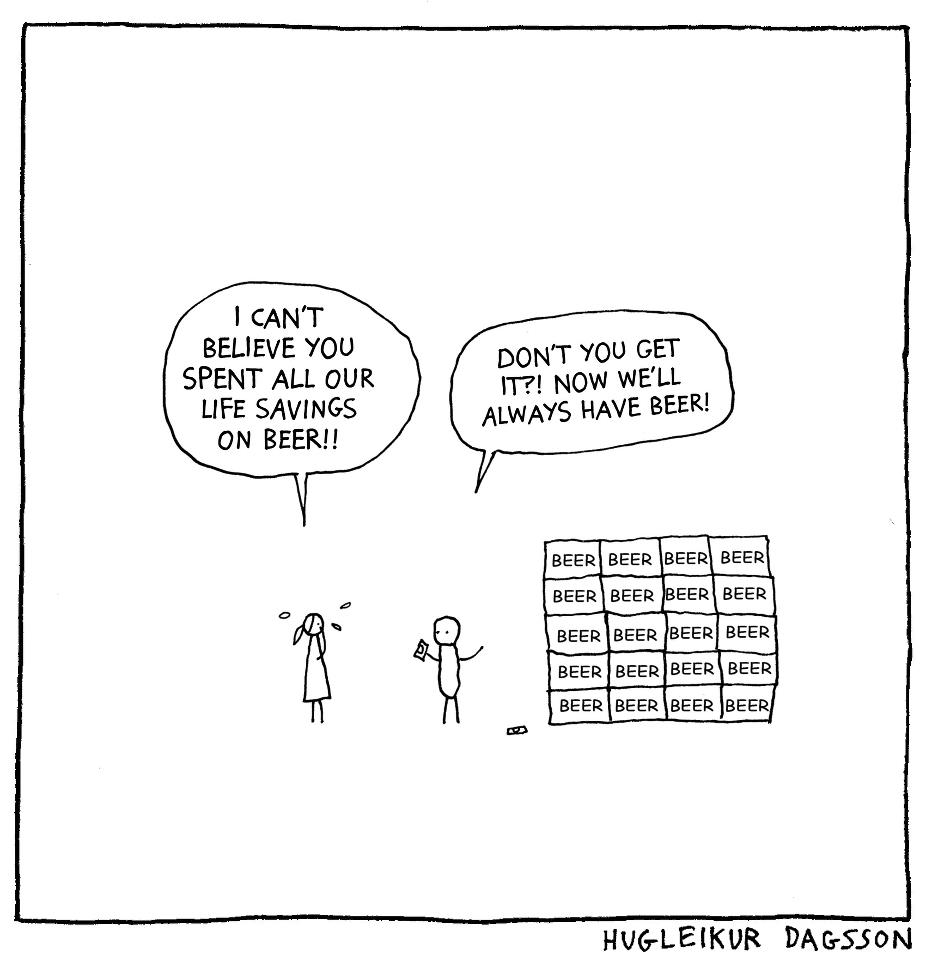
\includegraphics[scale=0.45]{Bilder/forside.jpg} %scale justerer størrelsen på bilde. Linjen etterpå er mappen bilde ligger i.
\end{figure}
    \ \\
    \ \\
        {\large
    Alcoholic Beverages Chart\\
    }
    \ \\
    {\today\ \\}
    \ \\
    \end{center}
    \end{titlepage}
    
    \thispagestyle{empty}
\newpage

\setcounter{page}{1}
\pagenumbering{arabic}
%her er innholdsfortegnelsen. Den lages automagisk
\tableofcontents
\newpage

%HER ER EN LITEN BRUKSANVISNING
%Nedenfor er en mal til hvordan man lager en subsubsection
\begin{comment}
%start å klipp og lim herifra, og lim det inn under riktig "subsection":

\subsubsection{Bryggeri: NAVN PÅ ØL}
\paragraph{Kommentar:} SKRIV DIN MENING HER
\newline
-- -- ( SKRIV NAVN OG DATO)

\begin{figure} [H] %[H] hindrer latex i å bestemme hvor bilde skal stå. men det kommer der du vil ha det.
\centering
\includegraphics[scale=0.60, angle=0]{Bilder/Øl/outcomeinterruption.png} %scale justerer størrelsen på bilde, angle rotasjonen. Linjen etterpå er mappen bilde ligger i.
\caption{SKRIV EN BILDE TEKST.}
\end{figure}
\newpage
%stopp med klipp og lim her! --------------------------
\end{comment}


\section{Øl}
\subsection{Bayer}

\subsubsection{Det Lille Bryggeriet: Bjønnøl}
\paragraph{Kommentar:}Kjedelig og smakløst øl. Lever ikke opp til navnet og er ikke verdt pengene.
\newline
-- -- Isak 13.04.2014

\begin{figure} [H]
\centering
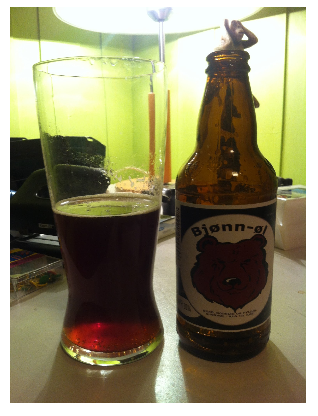
\includegraphics[scale=1.00]{Bilder/Ol/bjonnol.png} %scale justerer størrelsen på bilde. Linjen etterpå er mappen bilde ligger i.
\caption{Bjønnøl fra "Det Lille Bryggeri"}
\end{figure}

\newpage
\subsection{Ale}

\subsubsection{Ægir Bryggeri: Lindisfarne Scotch Ale}
\paragraph{Kommentar:}Ett meget godt øl med god rund smak. Hvis du er ute etter ett mørkt øl som passer godt med kjøttmat så er dette ett godt alternativ. Selv drakk jeg det sammen med gourmetpølser fra Jacob Aall og potetstappe og det funket veldig bra. Kunne helt fint vært ennå mørkere og kraftigere for min del, men så er jeg glad i mørkt øl.  
\newline
-- -- Isak 16.04.2014

\begin{figure} [H]
\centering
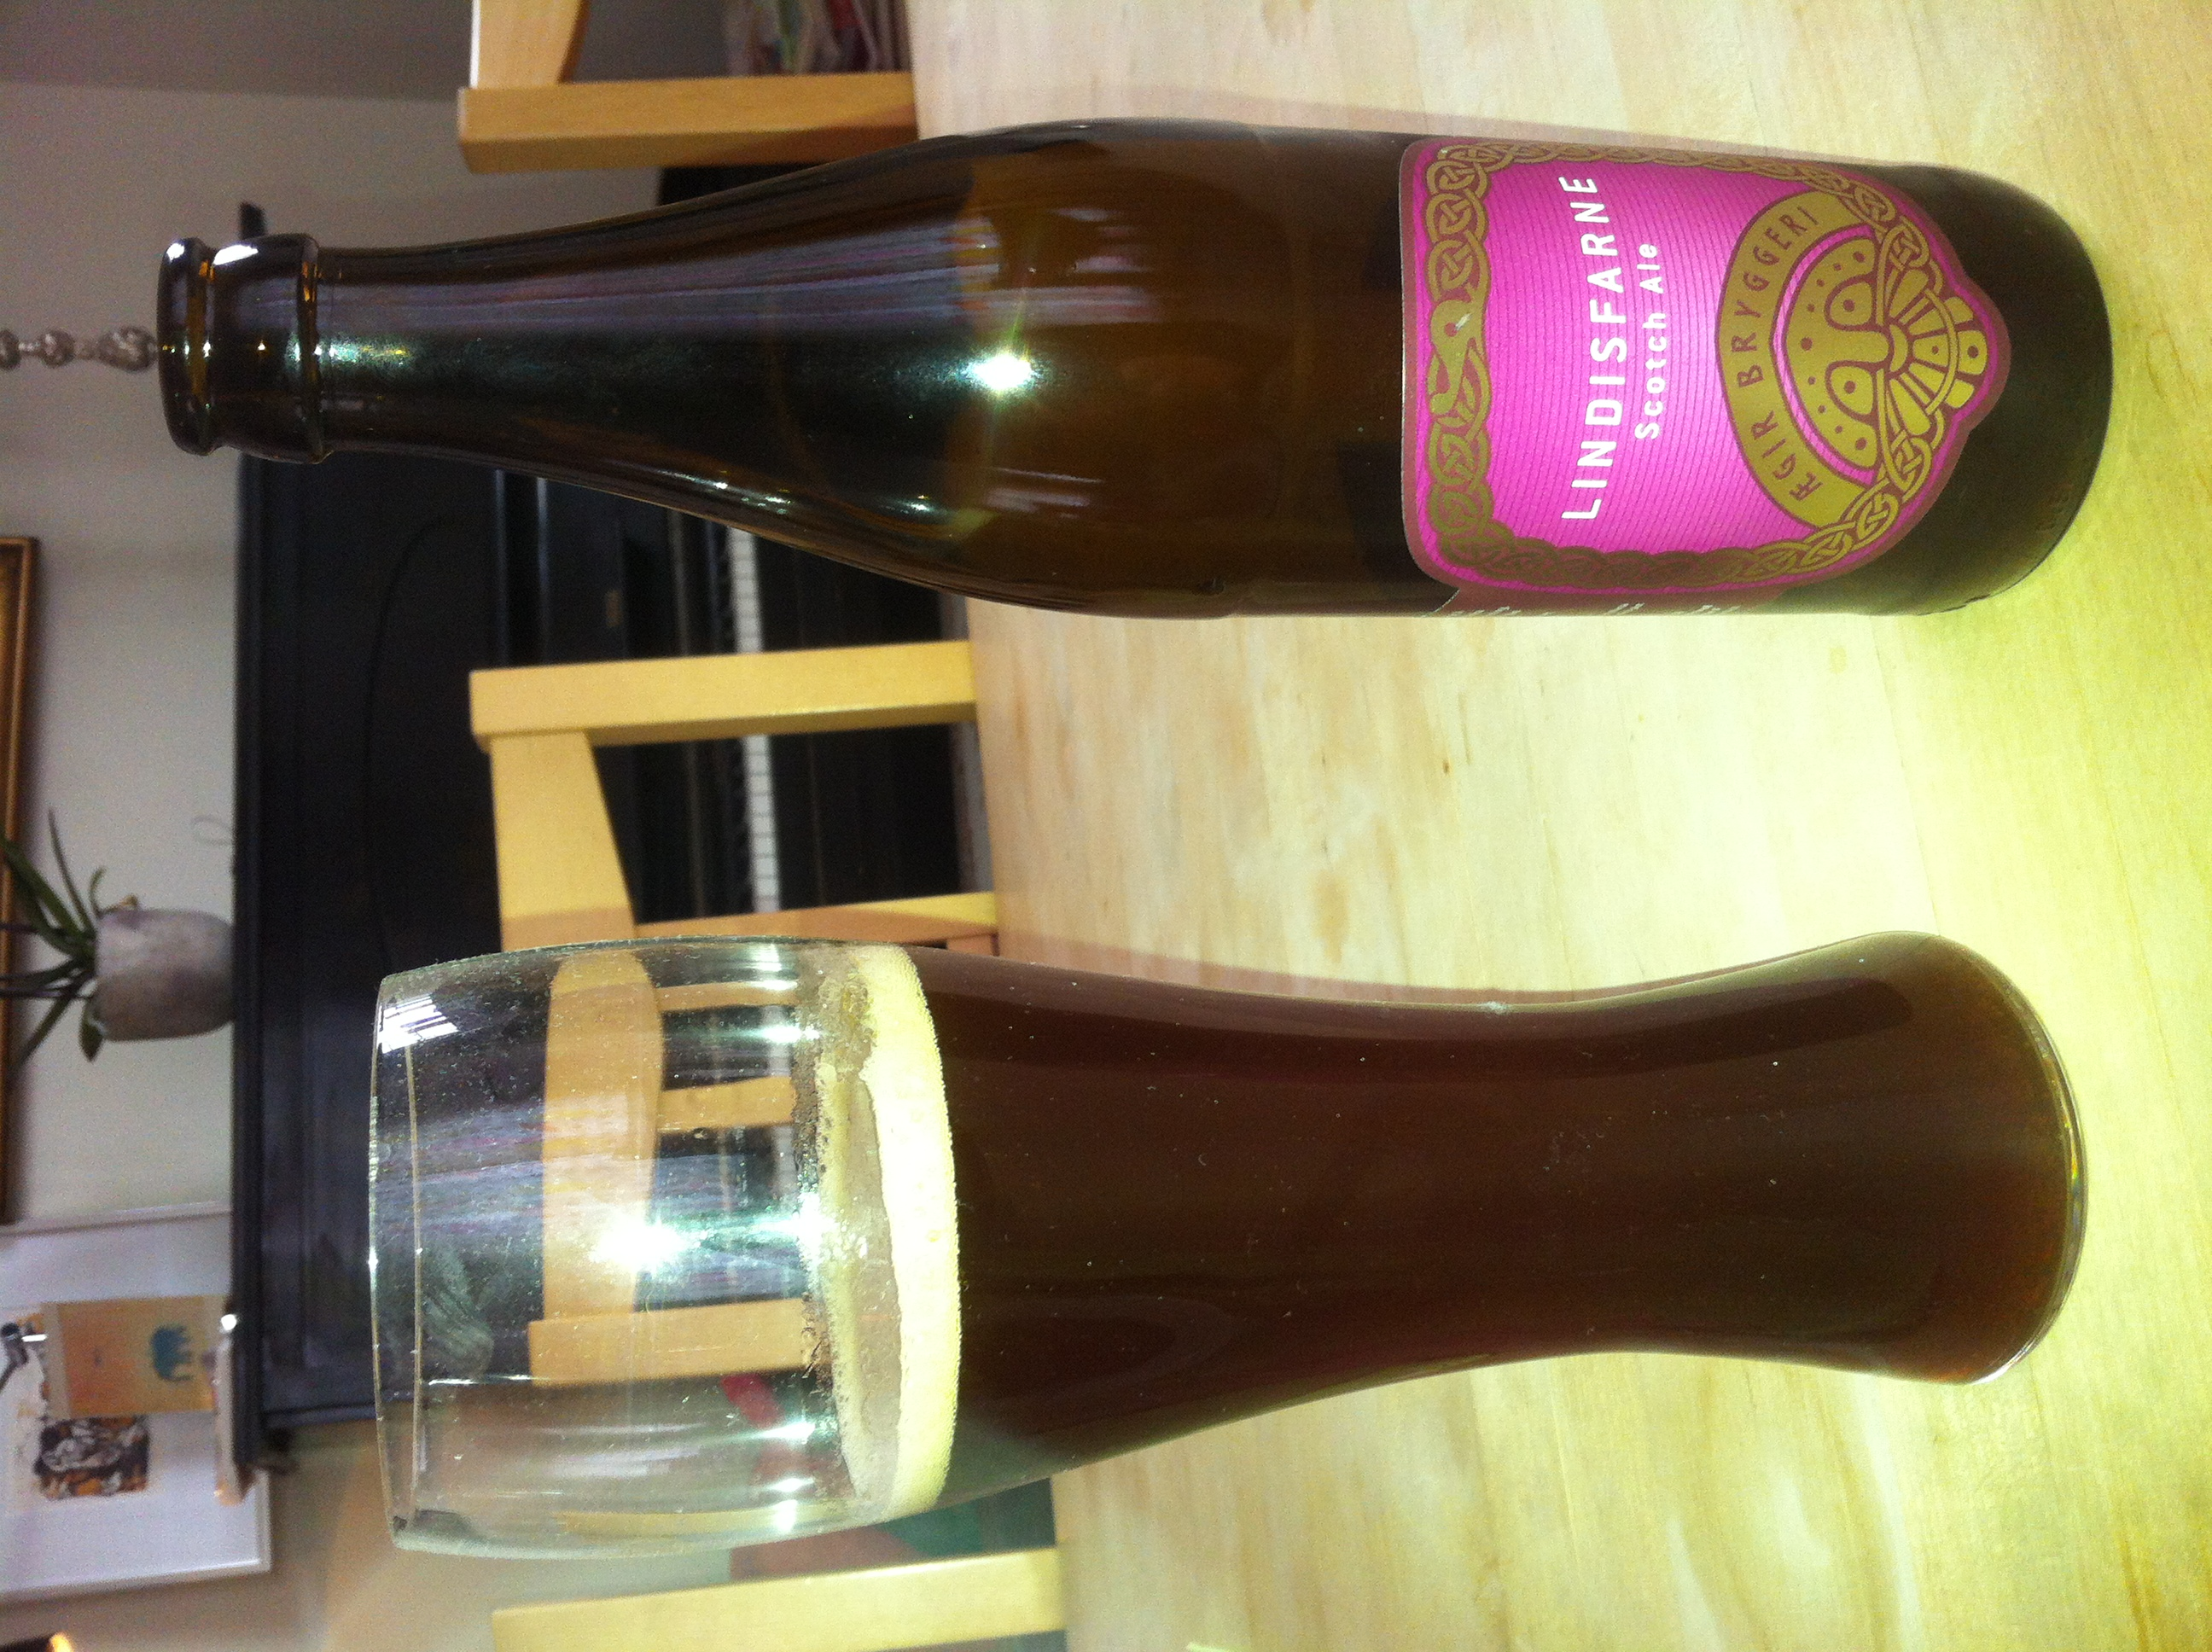
\includegraphics[scale=0.1, angle=270]{Bilder/Ol/lindisfarne}
\caption{Lindisfarne Scotch Ale fra Ægir Bryggeri}
\end{figure}

\newpage
\subsection{Pils}

\subsubsection{Det Lille Bryggeriet: Birkebeinerpils}
\paragraph{Kommentar:}Nok en skuffende øl fra Det Lille Bryggeriet. Kjedelig og en litt ubehagelig smak i svelget. 
\newline
-- -- Isak 13.04.2014

\begin{figure} [H]
\centering
\includegraphics[scale=0.1, angle=270]{Bilder/Ol/Birkebeiner.jpg}
\caption{Birkebeinerpils fra "Det Lille Bryggeriet"}
\end{figure}

\newpage
\subsubsection{E.C. Dahls Bryggeri: Dahls Pils}
\paragraph{Kommentar:}En ok industripils til prisen man betaler for den. Den har et preg av banan og fargen er som morgen-piss. Nytes best full, kan like gjerne drikkes rett fra flasken som fra glass. Da sparer man litt oppvask. Selv om ølen har et kipt industripreg, er den vist nok gunstig for bartevekst. Bivirkning ved ølen er utydelig tale og trang til å skyte inn med ordet "sjø" stadig vekk.
\newline
-- -- Anders 13.04.2014

\begin{figure} [H]
\centering
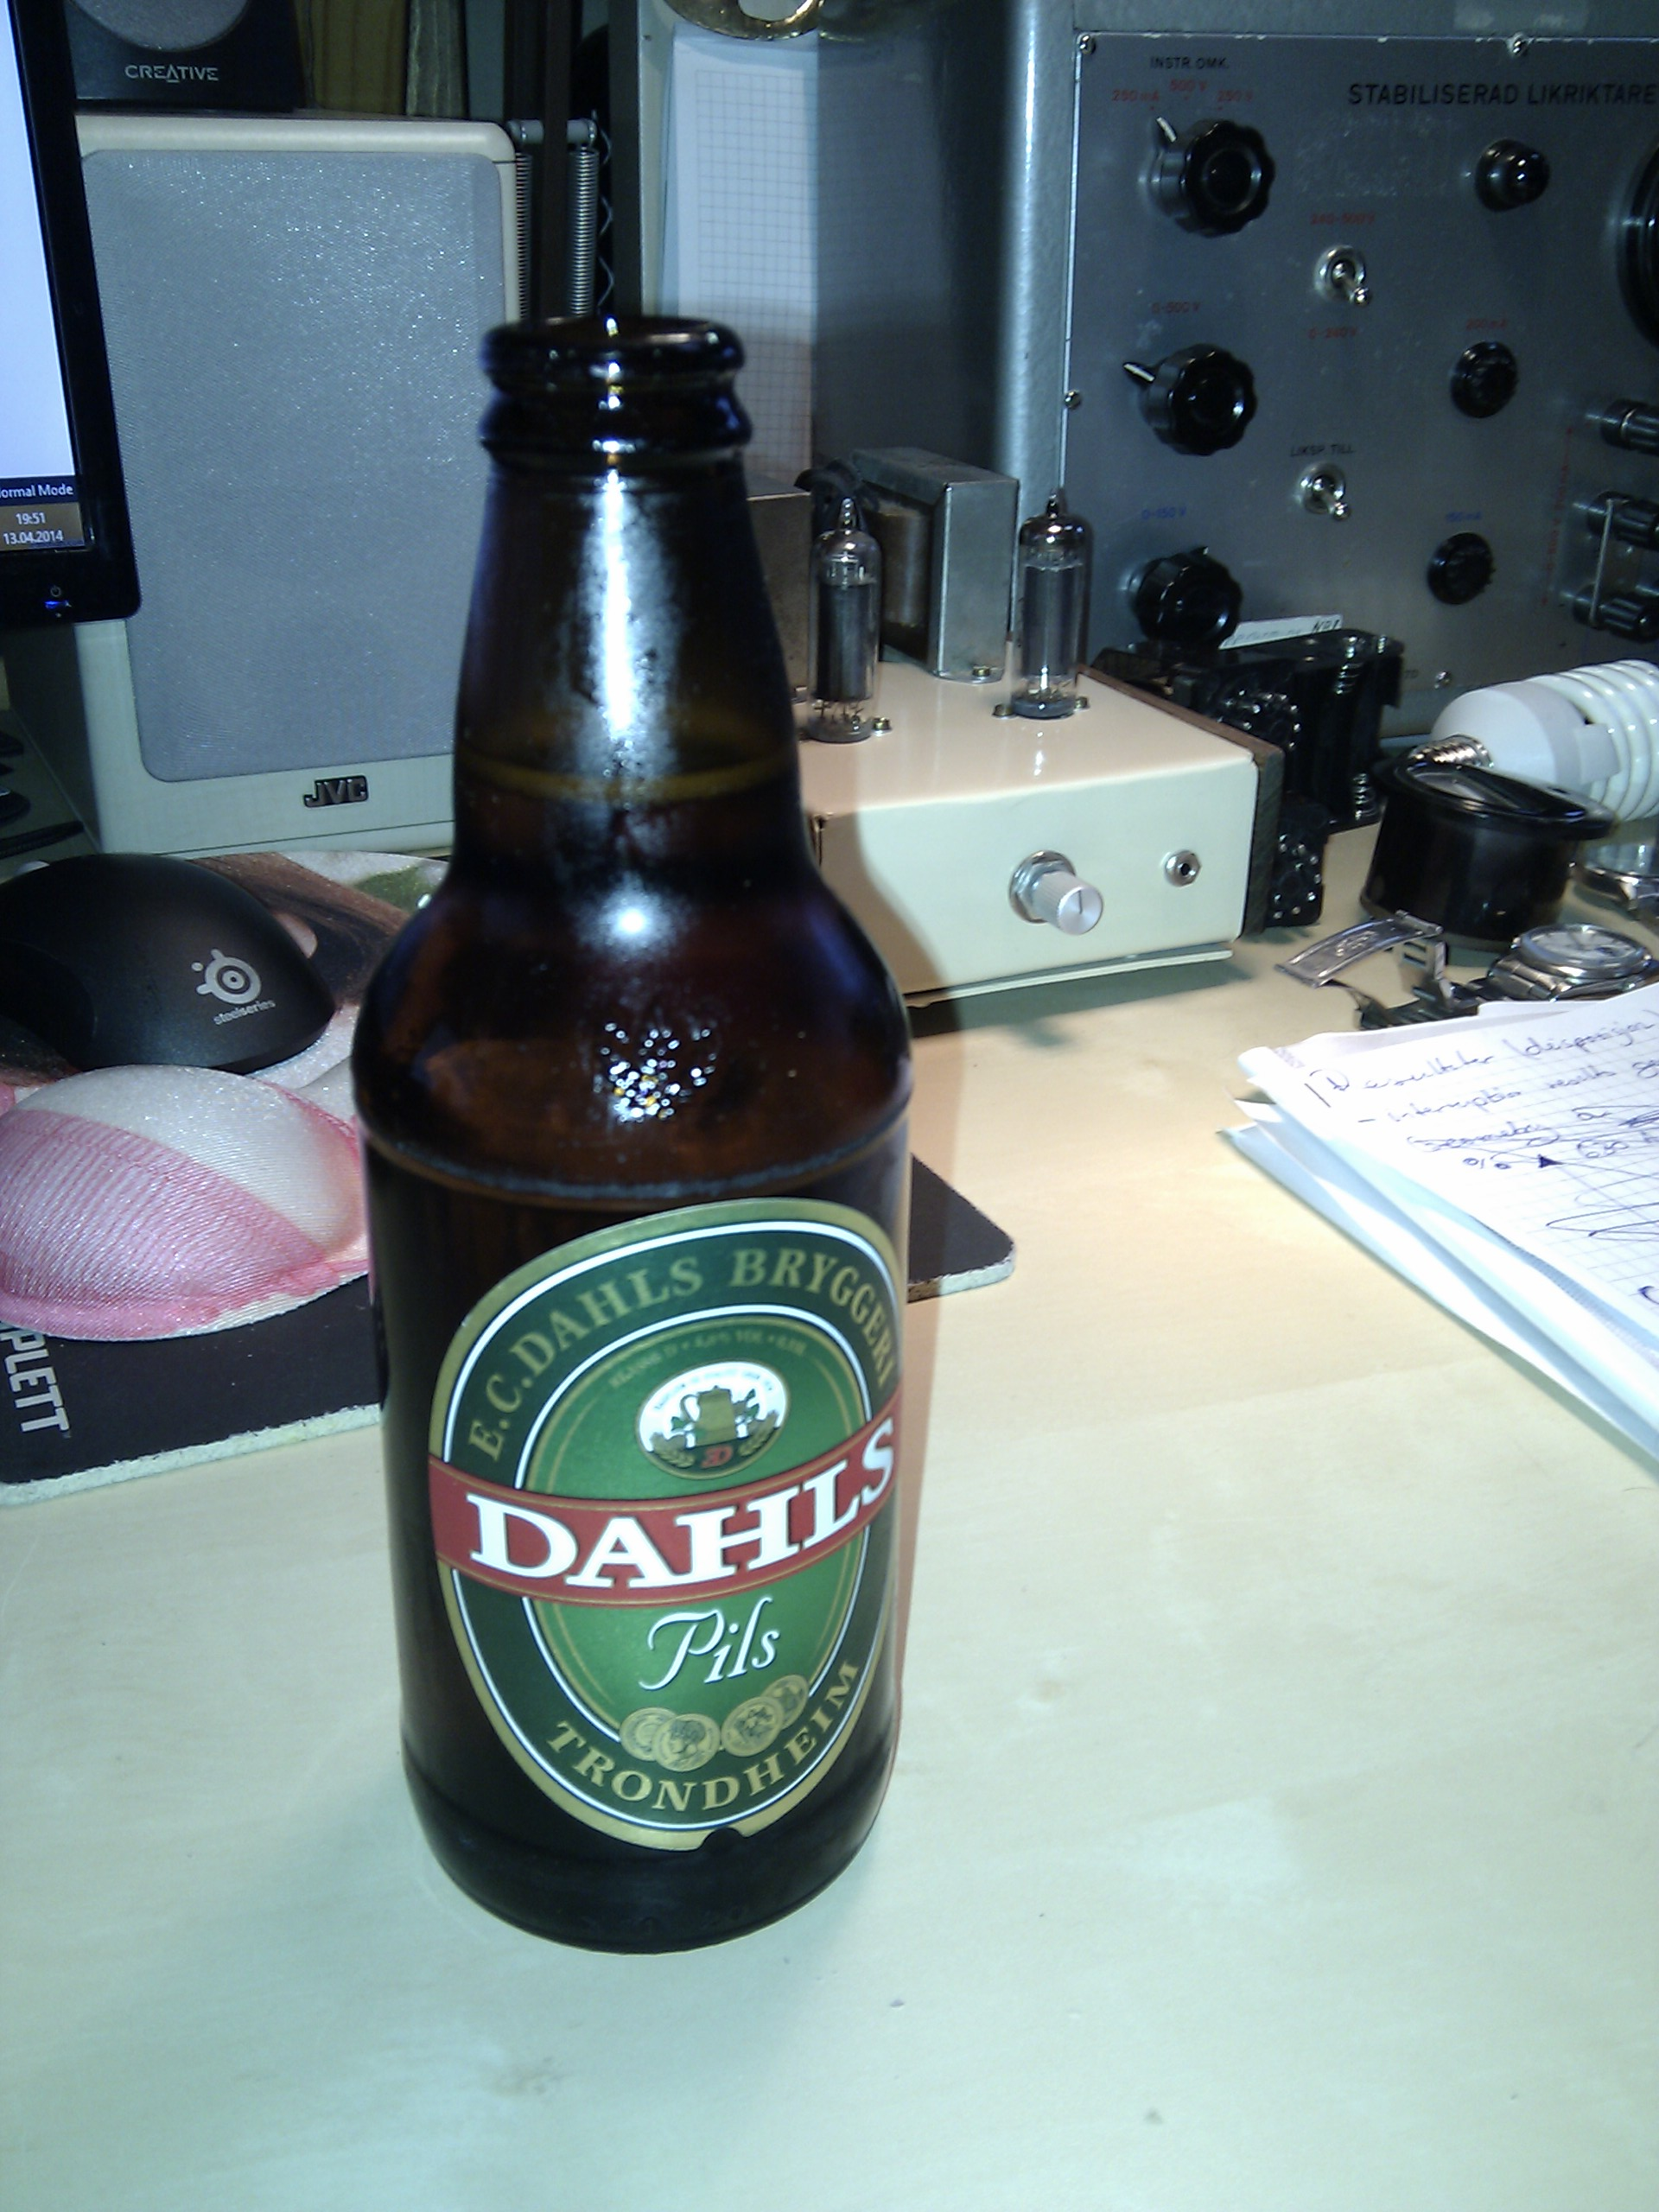
\includegraphics[scale=0.1, angle=0]{Bilder/Ol/dahls.jpg}
\caption{Dahls Pils fra "E.C. Dahls Bryggeri"}
\end{figure}

\newpage
\subsubsection{Nordlands Bryggeri: Nordlands Pils}
\paragraph{Kommentar:}Det er rart at man prøver å selge en sommerpils fra Nord-Norge. Det er svært lite sommerlig ved Nord-Norge. Som Dahlsen nytes denne også best full, kan like gjerne drikkes rett fra flasken som fra glass. På flasken står det at det er mye hygge i en nordlending. Det stemmer nok, men nordlendingen drikker nok Mack. Det kan være nordlendingen benytter seg av en knust flaske Nordlands Pils når de trenger stikkvåpen fordi hans fetteren nettopp dumpet hans søster til fordel for en russisk import-brud. Pilsen har et litt søtlig krydder preg over seg, og er veldig lys i fargen. Den er relativt smakløs nesten som vann, finnes sikkert noen som liker det å.
\newline
-- -- Anders 14.04.2014

\begin{figure} [H]
\centering
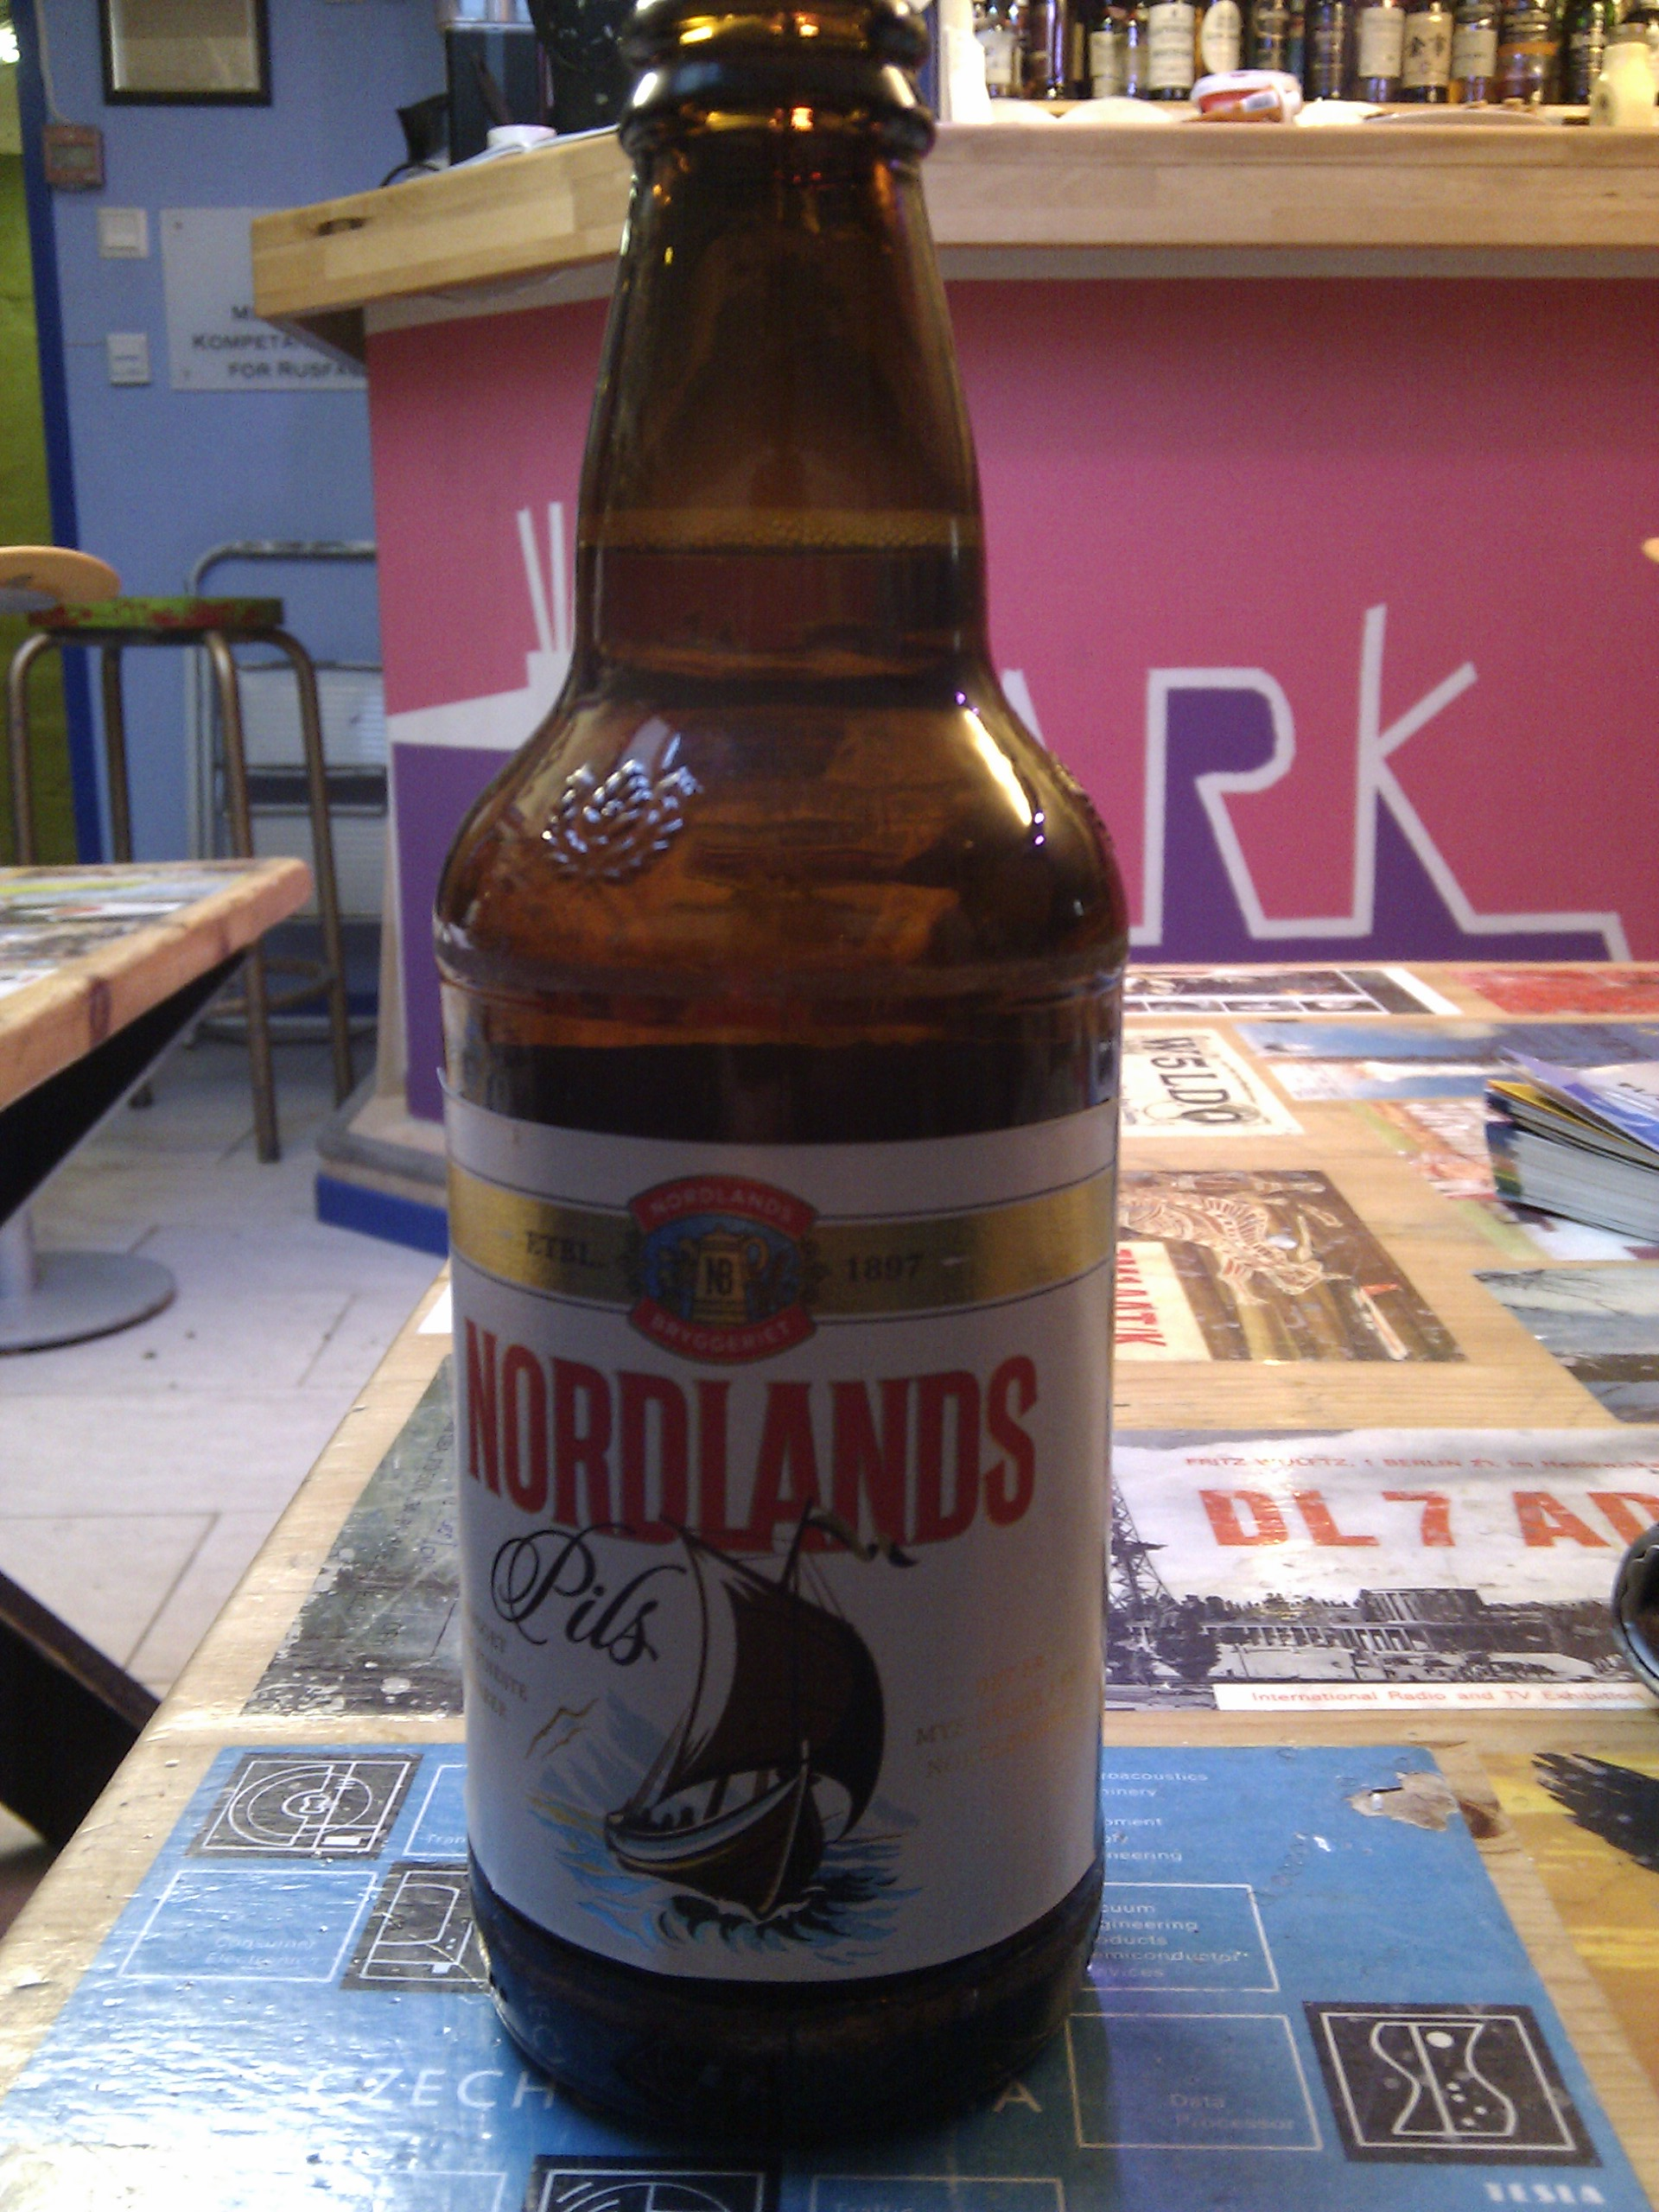
\includegraphics[scale=0.1, angle=0]{Bilder/Ol/NordlandsPils.jpg}
\caption{Nordlands Pils fra "Nordlands Bryggeri"}
\end{figure}

\newpage
\subsection{IPA}
\subsubsection{Austmann Bryggeri: Humledugg}
\paragraph{Kommentar:} Ikke blant de rammeste IPA'ene, men har som en IPA skal ha et tydelig bittert preg. Om jeg først skal kjøpe IPA, tror jeg at jeg ville gått for andre varianter enn denne, rett å slett fordi den er i det litt mildeste laget. Om man derimot har lyst på en bitter øl (men ikke IPA bitter) er dette et godt valg. Den er riktig nok dyr i forhold til mengden du får, 0,33 l for over 50 lappen på polet er ikke spesielt rimelig. Hadde jeg fått en halv liter til den prisen hadde det vært lettere å forsvare prisen i forhold til kvaliteten. Ølen er forøvrig noe lysere enn den fremstår på bilde.
\newline
-- -- Anders 16.04.2014

\begin{figure} [H]
\centering
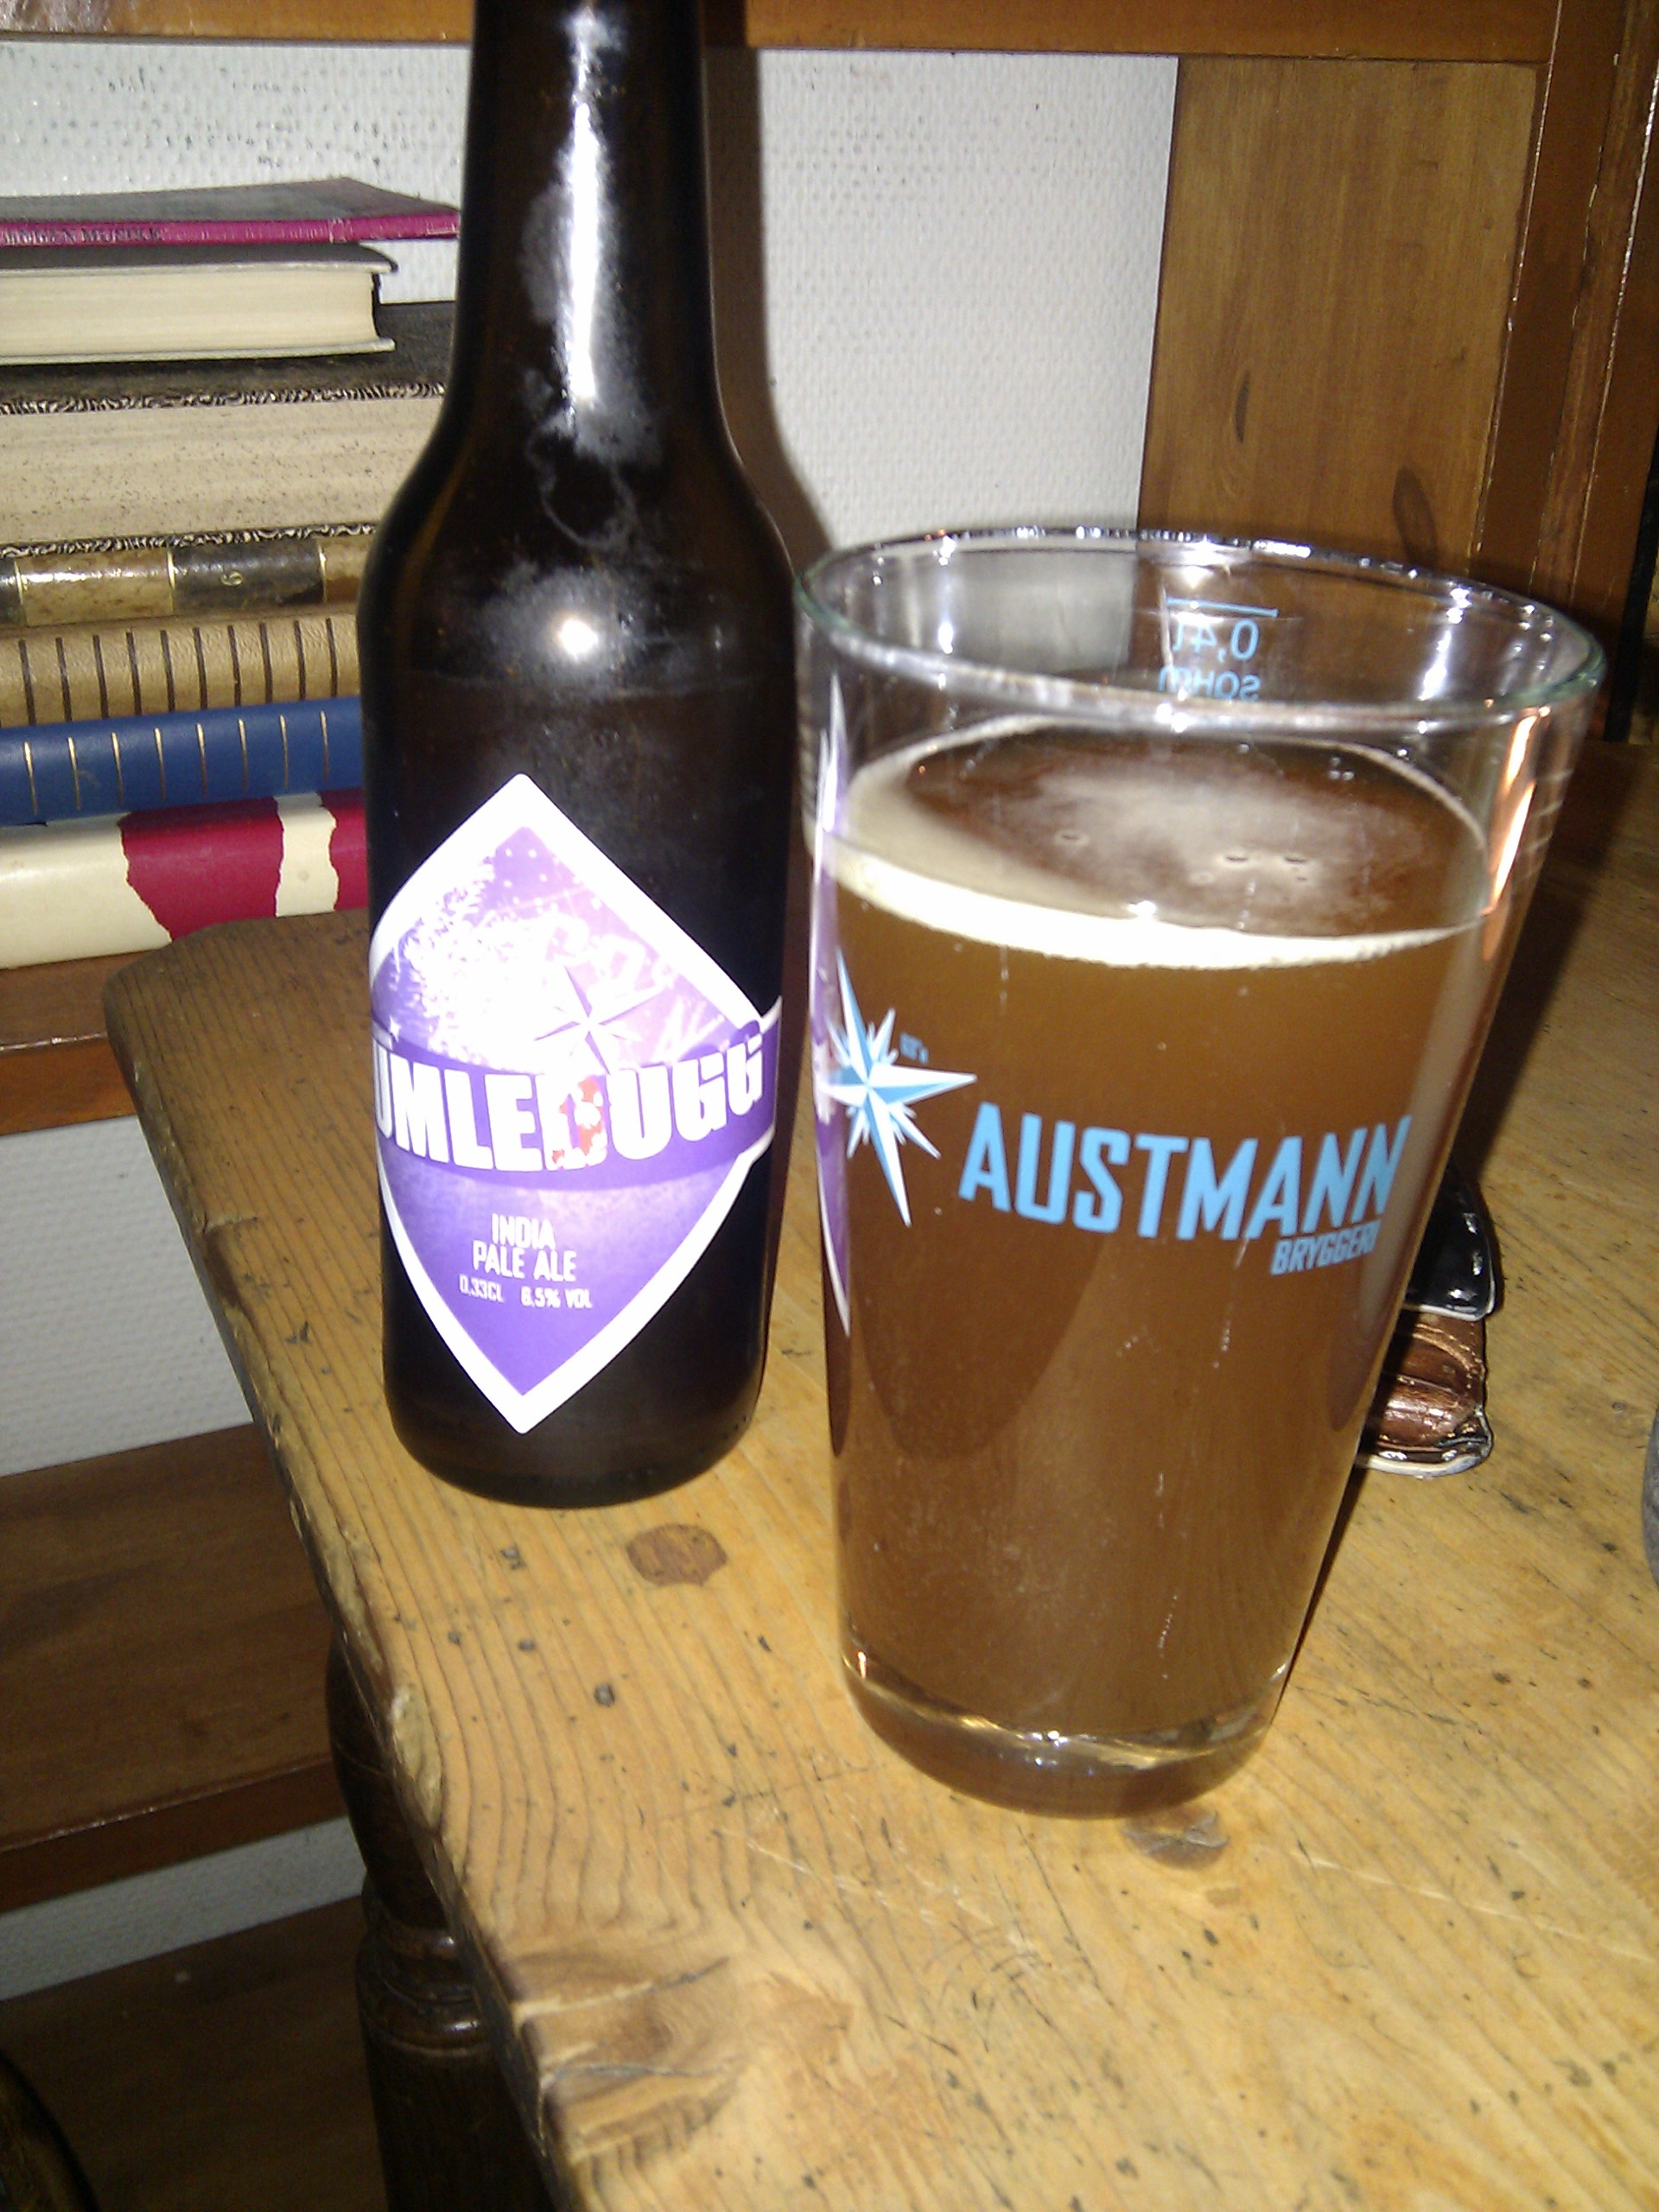
\includegraphics[scale=0.1, angle=0]{Bilder/Ol/humledugg.jpg}
\caption{Humledugg fra "Austmann Bryggeri"}
\end{figure}


\newpage
\subsection{Hveteøl}
\subsubsection{Ægir Bryggeri: Witbier}
\paragraph{Kommentar:} Til å være hveteøl var denne mindre søt enn jeg hadde forventet. Den var lett og lys, og egner seg kanskje i mer sommerlige situasjoner enn jeg drakk den i. Selv savnet jeg litt mer ramm smak, men det skal man kanskje ikke forvente av en hveteøl. Hadde jeg hatt valget mellom denne og en Dahls ville jeg tatt denne, så lenge jeg ikke måtte betale for den selv. For lite smak for pengene rett å slett.
\newline
-- -- Anders 14.04.2014

\begin{figure} [H]
\centering
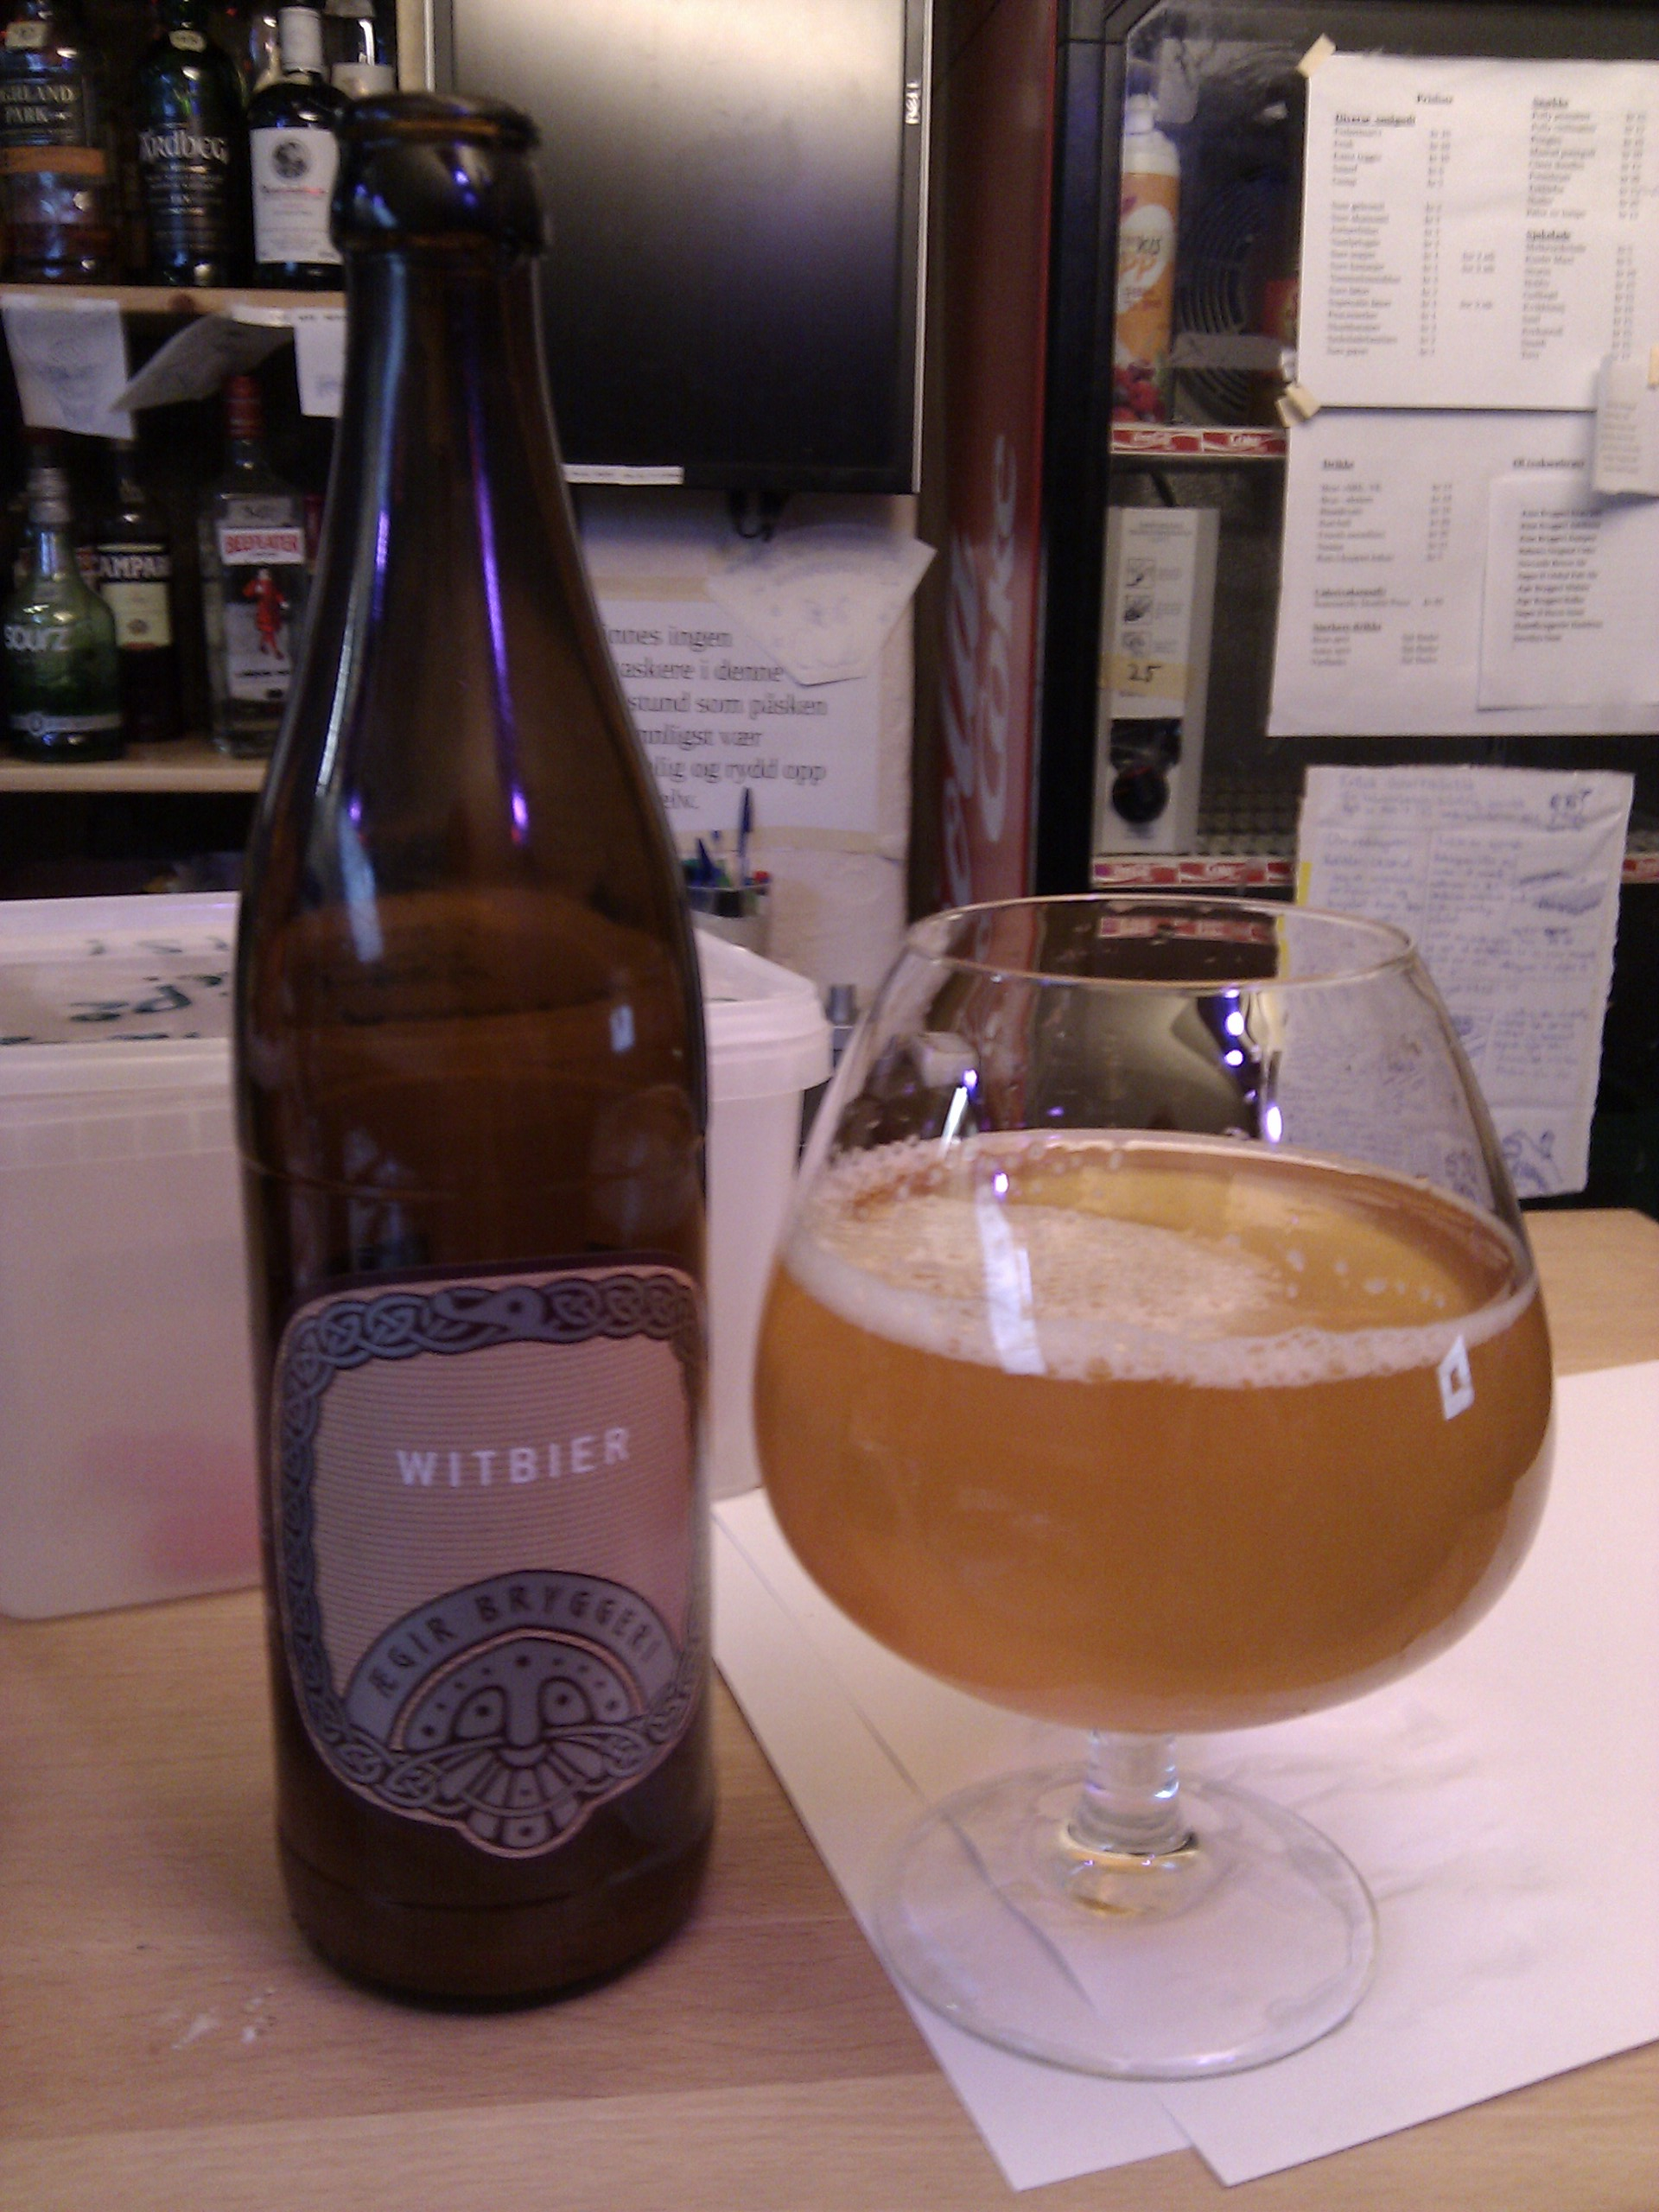
\includegraphics[scale=0.1, angle=0]{Bilder/Ol/EgirBryggeriWitbier.jpg}
\caption{Witbier fra "Ægir Bryggeri"}
\end{figure}

\newpage
\section{Vin}

\newpage
\section{Sprit}
\subsection{Whisky}
\subsubsection{Lagavulin: Island Single Malt Scotch Whisky 16 Years}

\paragraph{Kommentar:}Sterk, men behagelig røkpreg. En "varmende" avrunding, men ikke en typisk rund whisky. Til en middels høy pris på polet er dette verdt hver krone. Et må ha i barskapet. Plix ikke bland cola i dette a.
\newline
-- -- Anders 13.04.2014

\begin{figure} [H]
\centering
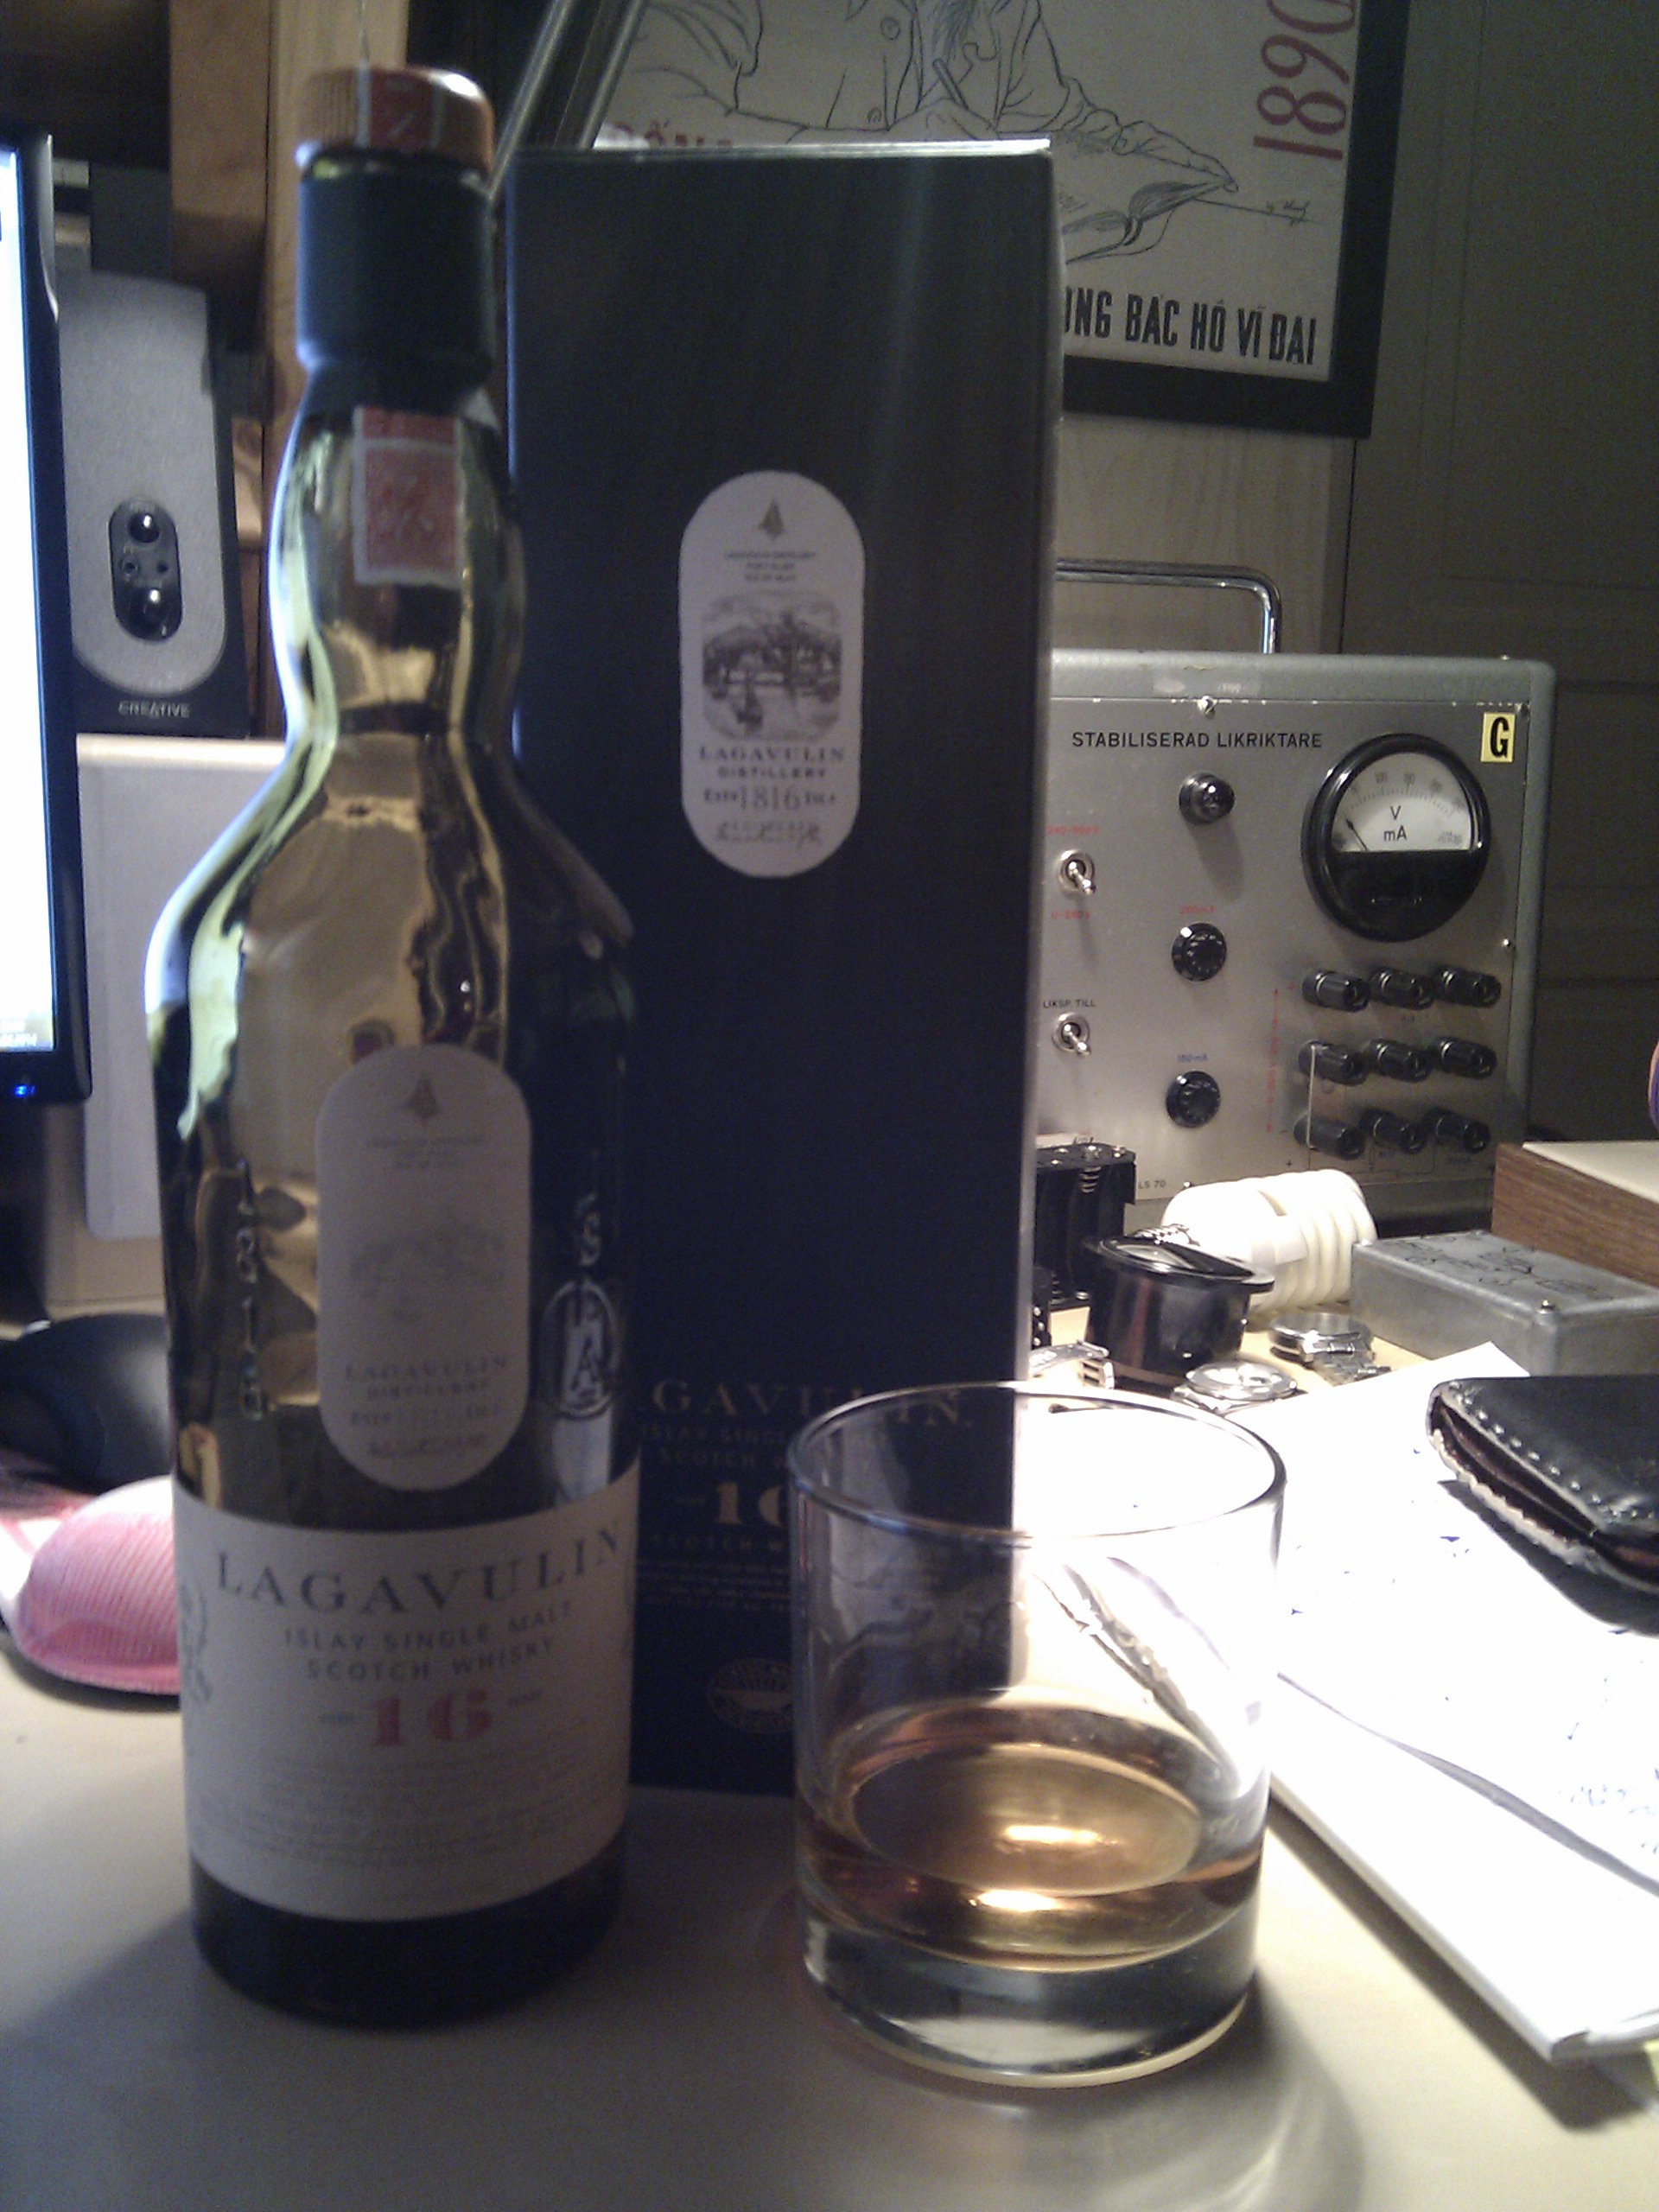
\includegraphics[scale=0.1, angle=0]{Bilder/Sprit/Lagavulin16aar.jpg}
\caption{Island Single Malt Scotch Whisky 16 Years fra "Lagavulin"}
\end{figure}


\newpage
\subsection{Cognac}
\end{document}